\documentclass[10pt]{article}
\usepackage{fullpage,graphicx,psfrag,amsmath,amsfonts,verbatim}
\usepackage[small,bf]{caption}

\newcommand{\ones}{\mathbf 1}
\newcommand{\reals}{{\mbox{\bf R}}}
\newcommand{\integers}{{\mbox{\bf Z}}}
\newcommand{\symm}{{\mbox{\bf S}}}  % symmetric matrices

\newcommand{\nullspace}{{\mathcal N}}
\newcommand{\range}{{\mathcal R}}
\newcommand{\Rank}{\mathop{\bf Rank}}
\newcommand{\Tr}{\mathop{\bf Tr}}
\newcommand{\diag}{\mathop{\bf diag}}
\newcommand{\card}{\mathop{\bf card}}
\newcommand{\rank}{\mathop{\bf rank}}
\newcommand{\conv}{\mathop{\bf conv}}
\newcommand{\prox}{\mathbf{prox}}

\newcommand{\Expect}{\mathop{\bf E{}}}
\newcommand{\Prob}{\mathop{\bf Prob}}
\newcommand{\Co}{{\mathop {\bf Co}}} % convex hull
\newcommand{\dist}{\mathop{\bf dist{}}}
\newcommand{\argmin}{\mathop{\rm argmin}}
\newcommand{\argmax}{\mathop{\rm argmax}}
\newcommand{\epi}{\mathop{\bf epi}} % epigraph
\newcommand{\Vol}{\mathop{\bf vol}}
\newcommand{\dom}{\mathop{\bf dom}} % domain
\newcommand{\intr}{\mathop{\bf int}}
\newcommand{\sign}{\mathop{\bf sign}}

\newcommand{\cf}{{\it cf.}}
\newcommand{\eg}{{\it e.g.}}
\newcommand{\ie}{{\it i.e.}}
\newcommand{\etc}{{\it etc.}}
\bibliographystyle{alpha}

\title{Problem sets for MATH 312}
\author{Ashok M. Rao}

\begin{document}
\maketitle

\section{Homework 1}
\subsection{(Strang 1.1.2)}
See figure 1. (I could not make the arrows in time but they are radially outward). 
\begin{figure}
\begin{center}
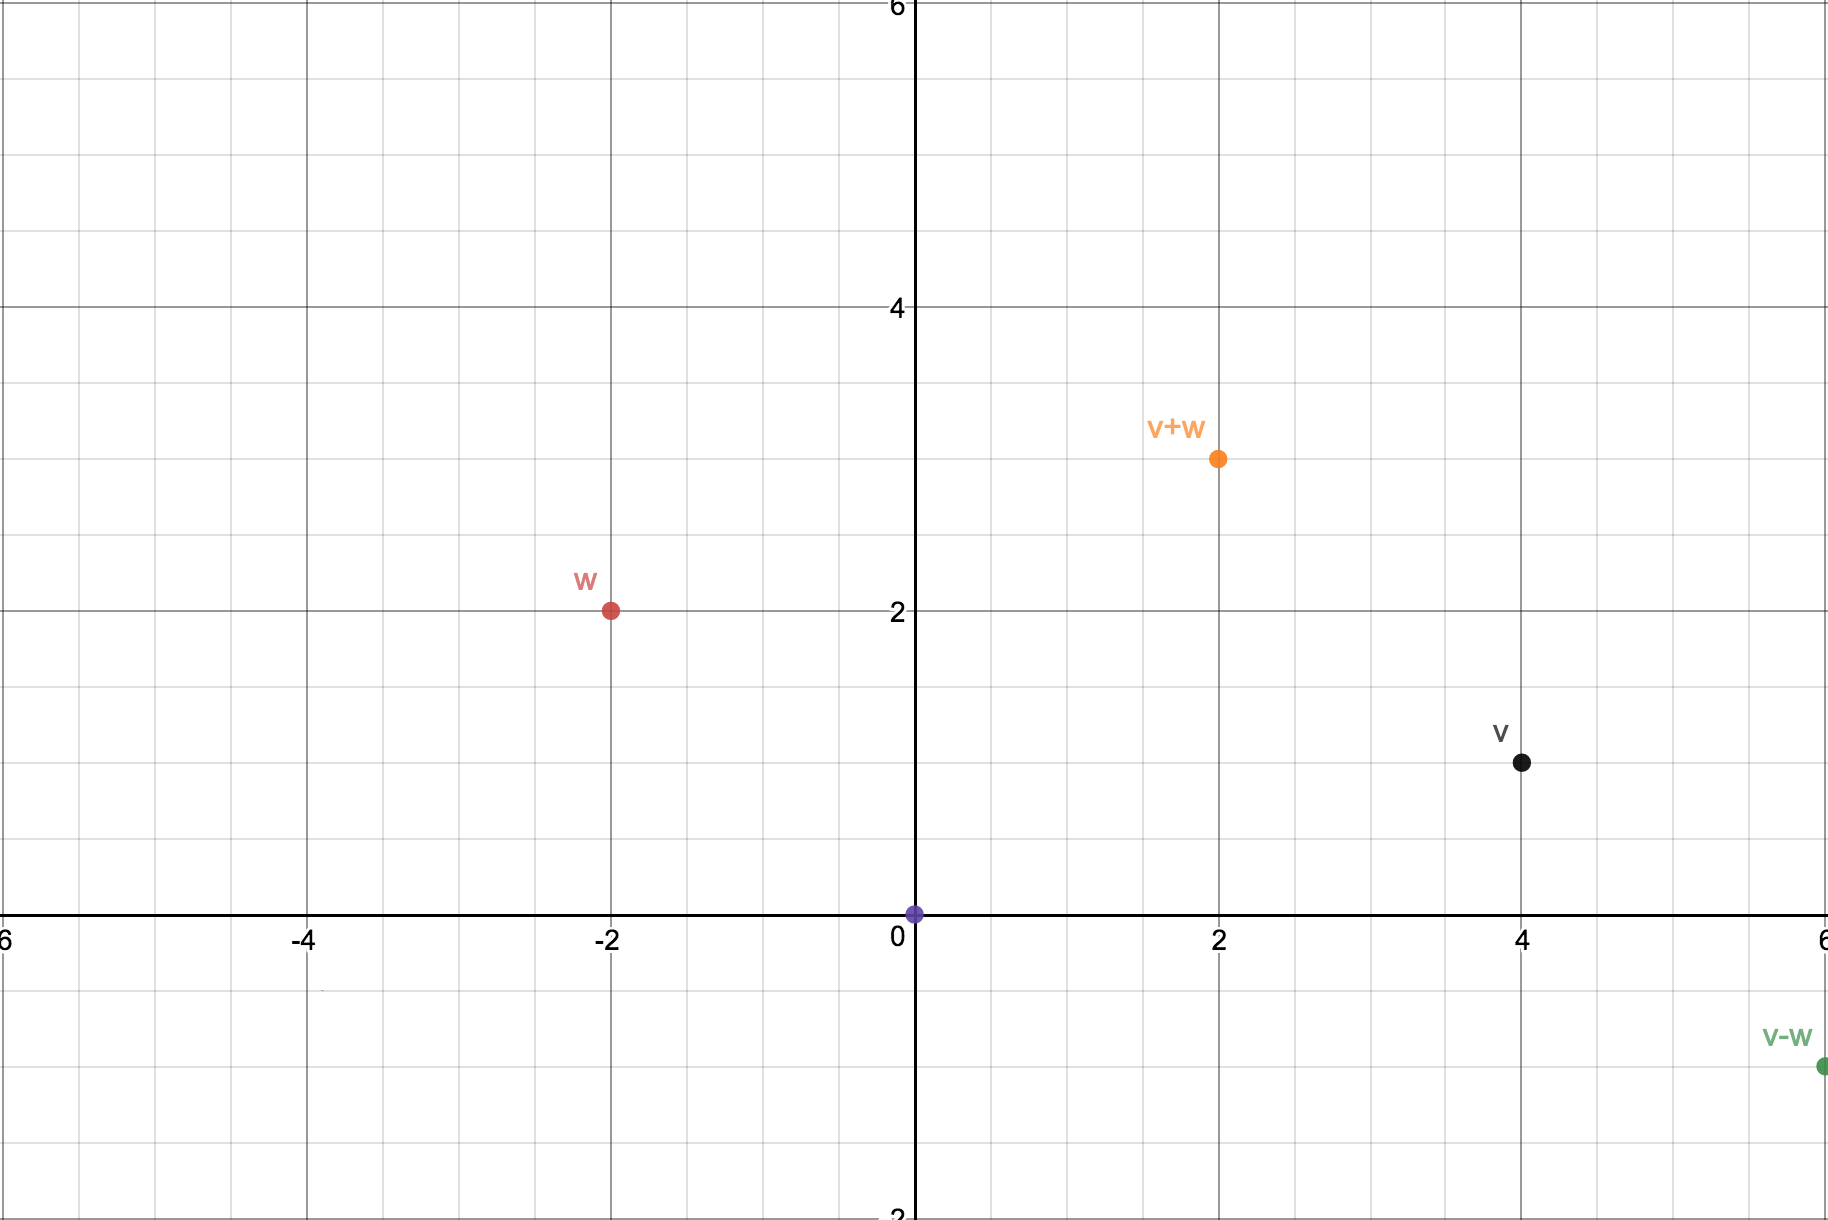
\includegraphics[width=0.6\textwidth]{ss1}
\end{center}
\caption{Vectors as labeled}
\end{figure}

\subsection{(Strang 1.1.18)}
Let me pick $e_1$ and $e_2$ in $\reals^2$. Linear combinations over positive coefficients would then yield the square shaded over $\{0, 1\}\times\{0, 1\}$. See figure 2.
\begin{figure}
\begin{center}
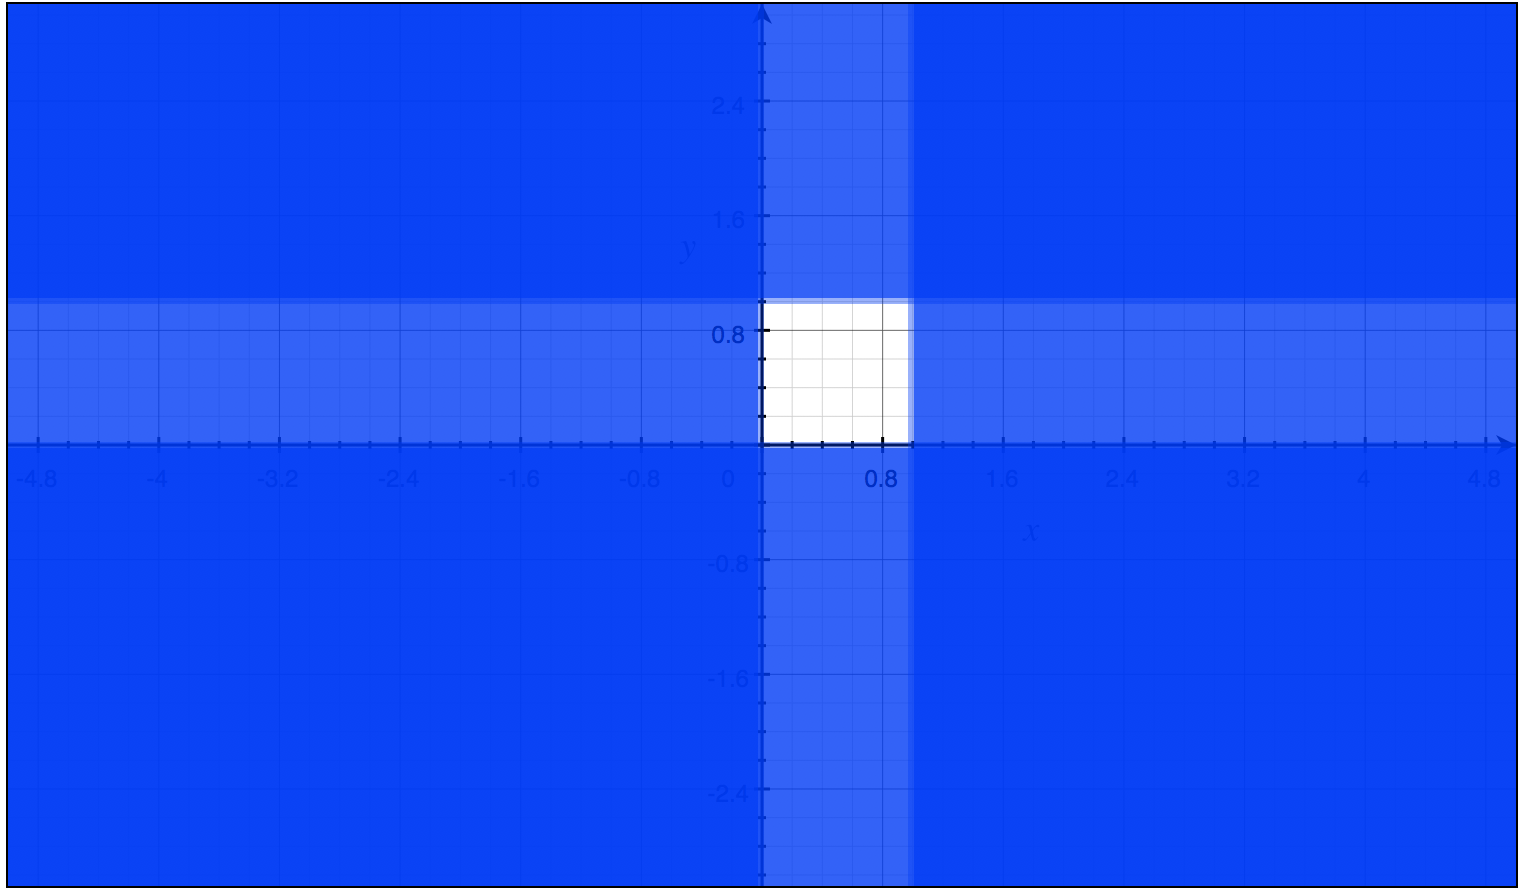
\includegraphics[width=0.6\textwidth]{ss2}
\end{center}
\caption{The unshaded area is the span of linear combinations}
\end{figure}

\subsection{(Strang 1.2.7)}
The inner product between two vectors returns the (normalized) cosine of the angle subtended thereof.  So
\begin{enumerate}
	\item $\theta_a = \arccos{1/2}$, 60 degrees.
	\item $\theta_b = \arccos{0}$, 90 degrees.
	\item $\theta_c = \arccos{1/2}$, 60 degrees.
	\item $\theta_d = \arccos{1/\sqrt{2}}$, 135 degrees. 
\end{enumerate}

\subsection{(Strang 1.2.13)}
Flipping bits across the $z$-axis, vectors $(0, 1, 0)$ and $(1, 0, -1)$ are orthogonal to each other and the given vector $(1, 0, 1)$.

\subsection{(Strang 1.2.14)}
Flipping bits like above, so that there are an even number of zero coordinates on each vector, we first have $(1, 1, -1, -1)$, and then $(0, 0, 1, -1)$ and $(1, -1, 0, 0)$, as possibilities. 

\subsection{Linear independence of three vectors}
No. ${\bf u} + {\bf w} = 2{\bf v}$.

\subsection{(Strang 1.3.14)}
This follows from cross multiplication. Whenever $(a, b)$ is a multiple of $(c, d)$ we have $a/c = b/d$ and thus it must be that $a/b = c/d$. 

\section{Homework 2}
\subsection{(Strang 2.1.16)}
A matrix $R$ rotates a vector $x\in \reals^2$ by $\theta$ degrees if $\langle x, Rx \rangle = (x^2 + y^2)\cos{\theta}$. Not quite guessing possible candidates in the dark, let $x_r = x\cos{\theta} - y\sin{\theta}$ and $y_r = x\sin{\theta} + y\cos{\theta}$, \eg 
\[R(\theta) = 
\begin{bmatrix}
	\cos{\theta} & -\sin{\theta} \\
	\sin{\theta} & \cos{\theta}	
\end{bmatrix}
\]
Clearly now $\langle x, Rx \rangle = (x^2 + y^2)\cos{\theta}$ providing the desired result. In clockwise terms then,
\[R(-90\text{ degrees}) = 
\begin{bmatrix}
	0 & 1 \\
	-1 & 0	
\end{bmatrix},\quad 
R(180\text{ degrees}) = 
\begin{bmatrix}
	-1 & 0 \\
	0 & -1	
\end{bmatrix}
\]
The latter result is more obviously interpreted as $-I$.

\subsection{Triangular elimination}
The system of equations to be solved is,
\begin{align*}
	2x_1 + 3x_2 &= 1 \\
	10x_1 + 9x_1 &= 11
\end{align*}
so $A = \begin{bmatrix}2 & 3\\ 10 & 9\end{bmatrix}$ and from $r_2 \leftarrow r_2 - 5r_1$ we get the system,
\[ 
\begin{bmatrix}2& 3\\0&-6\end{bmatrix}\begin{bmatrix}x_1\\x_2\end{bmatrix} = \begin{bmatrix}1\\6\end{bmatrix}\]
yielding $x = [2\quad -1]^T$.

\subsection{(Strang 2.2.13)}
The triangular matrix is 
\[
\begin{bmatrix}
	2& -3& 0\\
	4& -5& 1\\
	2& -1&-3
\end{bmatrix}\begin{bmatrix}3\\7\\5\end{bmatrix} \rightarrow
\begin{bmatrix}
	2& -3& 0\\
	0& 1& 1\\
	0& 0& -5
\end{bmatrix}\begin{bmatrix}3\\1\\0\end{bmatrix}
\]
following row operations
\begin{align*}
	r_2' \leftarrow r_2 - 2r_1 \\
	r_3' \leftarrow r_3 - r_1 - 2r_2'
\end{align*}
which gives $x = (3,1,0)$ as the solution.

\subsection{(Strang 2.3.17)}
The constraints here define the system
\[
\begin{bmatrix}1& 1& 1\\ 1& 2& 4\\ 1& 3& 9\end{bmatrix}\begin{bmatrix}a\\b\\c\end{bmatrix}=
\begin{bmatrix}4\\8\\14\end{bmatrix}
\]
With row operations,
\[
\begin{bmatrix}1& 1& 1\\ 1& 2& 4\\ 1& 3& 9\end{bmatrix}\begin{bmatrix}4\\8\\14\end{bmatrix}\rightarrow
\begin{bmatrix}1& 1& 1\\ 0& 1& 3\\ 0& 2& 8\end{bmatrix}\begin{bmatrix}4\\4\\10\end{bmatrix}\rightarrow
\begin{bmatrix}1& 1& 1\\ 0& 1& 3\\ 0& 0& 2\end{bmatrix}\begin{bmatrix}4\\4\\2\end{bmatrix}
\]
And so $a=2, b=1$ and $c=1$.

\subsection{(Strang 2.3.25)}
In the given matrix $A_3 = A_1 + A2$ and quite obviously $b_1 + b_2 \neq b_3$. Thus row operations would get you as far as $0 = 3$. Letting $b_{3}' = b_1 + b_2$ would reduce the system to the rectangular matrix defined on any two of the three rows, with infinitely many solutions. 

\subsection{(Strang 2.3.28)}
We have $AB = I$ and $BC = I$. By the definition of $I$, $A = A(BC)$ and $C = (AB)C$ and thus $A = C$ holds by the associative property.

\section{Homework 3}
\subsection{(Strang 2.4.15)}
\begin{enumerate}
\item True, otherwise rows and columns don't match or commute.
\item False, $AB$ need not equal $BA$ and they may have different sizes. ($m\times m$ and $n\times n$).
\item True, since inner dimensions agree on both.
\item False, let $B=0$ as counterexample.
\end{enumerate}

\subsection{(Strang 2.5.10)}
For $A$ the inverse follows just by logic of matrix multiplication and $B$ is block diagonal,
\[A^{-1} = \begin{bmatrix}0& 0& 0& 1/5\\0& 0& 1/4& 0\\0& 1/3& 0& 0\\1/2& 0&0 &0\end{bmatrix},\quad B^{-1} = \begin{bmatrix}3& -2& 0& 0\\-4& 3&0&0\\0&0&6&5\\0&0&7&6\end{bmatrix}\]

\subsection{(Strang 2.5.25)}
For $B$ notice that the all-ones vector is in the nullspace and thus no inverse exists. To invert $A$, first swap rows 1 and 2 and then eliminate
\[
\begin{bmatrix}	
1& 2& 1&    0&1& 0\\
0& -1& 1&   0&-1& 1\\
0& 0& -4&   1&1& -3
\end{bmatrix},\quad
\begin{bmatrix}	
1& 0& 0&    3/4&-1/4& -1/4\\
0& 1& 0&   -1/4&3/4 &-1/4\\
0& 0& 1&  -1/4& -1/4 &3/4
\end{bmatrix}
\]
Thus the answer becomes 
\[A^{-1} = \frac{1}{4}
\begin{bmatrix}
3& -1& -1 \\
-1&3&-1\\
-1&-1&3	
\end{bmatrix}
\]

\subsection{(Strang 2.6.13)}
By inspection, $L$ is a lower triangular matrix of ones and $U$ is upper triangular of $a$, then $b-a$, then $c-b$, and finally $d-c$. Specifically,
\[A = \begin{bmatrix}
 1& 0& 0& 0\\
 1& 1& 0& 0\\
 1& 1& 1& 0\\
 1& 1& 1& 1	
 \end{bmatrix}\begin{bmatrix}
a& a& a& a\\
0& b-a& b-a& b-a\\
0& 0& c-b& c-b&\\
0&0&0&d-c	
\end{bmatrix}
\]

\subsection{(Strang 2.7.16)}
For $A$, we swap rows 1 and 2,
\[
\begin{bmatrix}
	0& 1& 0\\
	1& 0& 0\\
	0& 0& 1\\
\end{bmatrix}A=
\begin{bmatrix}
	1& 0& 0\\
	0& 1& 0\\
	2& 3& 1\\
\end{bmatrix}
\begin{bmatrix}
	1& 0& 1\\
	0& 1& 1\\
	0& 0& -1\\
\end{bmatrix}
\]
And for $B$ we swap rows 2 and 3,
\[
\begin{bmatrix}
	1& 0& 0\\
	0& 0& 1\\
	0& 1& 0\\
\end{bmatrix}B=
\begin{bmatrix}
	1& 0& 0\\
	1& 1& 0\\
	2& 0& 1\\
\end{bmatrix}
\begin{bmatrix}
	1& 2& 0\\
	0& -1& 1\\
	0& 0& 1\\
\end{bmatrix}
\]

\subsection{Question about linearly independent vectors}
Yes. The matrix formed by these vectors are diagonally-dominant and thus invertible.
\end{document}